\documentclass[11pt]{article}

\usepackage[a4paper, left=1in, bottom=1in]{geometry}
\thispagestyle{empty}
\usepackage{pdfpages}
\usepackage{tikz}
\usepackage{listings}
\usepackage{minted}

\begin{document}

\includepdf[pagecommand={
	\begin{tikzpicture}[remember picture, overlay]
		\node at (2,-4.1) {del Mazo, Federico};
		\node at (8,-4.1) {100029};
		\node at (13,-4.1) {18/10/2020};
	\end{tikzpicture}}]{Parcialito3-Enunciado}

\begin{minted}[mathescape=true,escapeinside=||,breaklines,frame=single]{text}
peliculas_siglo_pasado = |$\rho$| movie_id |$\leftarrow$| id (|$\sigma$| movies.year < 2000 movies)
id_spielberg = |$\rho$| director_id |$\leftarrow$| id (|$\sigma$| directors.first_name = 'Steven' |$\land$|  directors.last_name = 'Spielberg' directors)
peliculas_spielberg = id_spielberg |$\bowtie$| movies_directors

peliculas_siglo_pasado |$\bowtie$| peliculas_spielberg
\end{minted}

\begin{figure}[H]
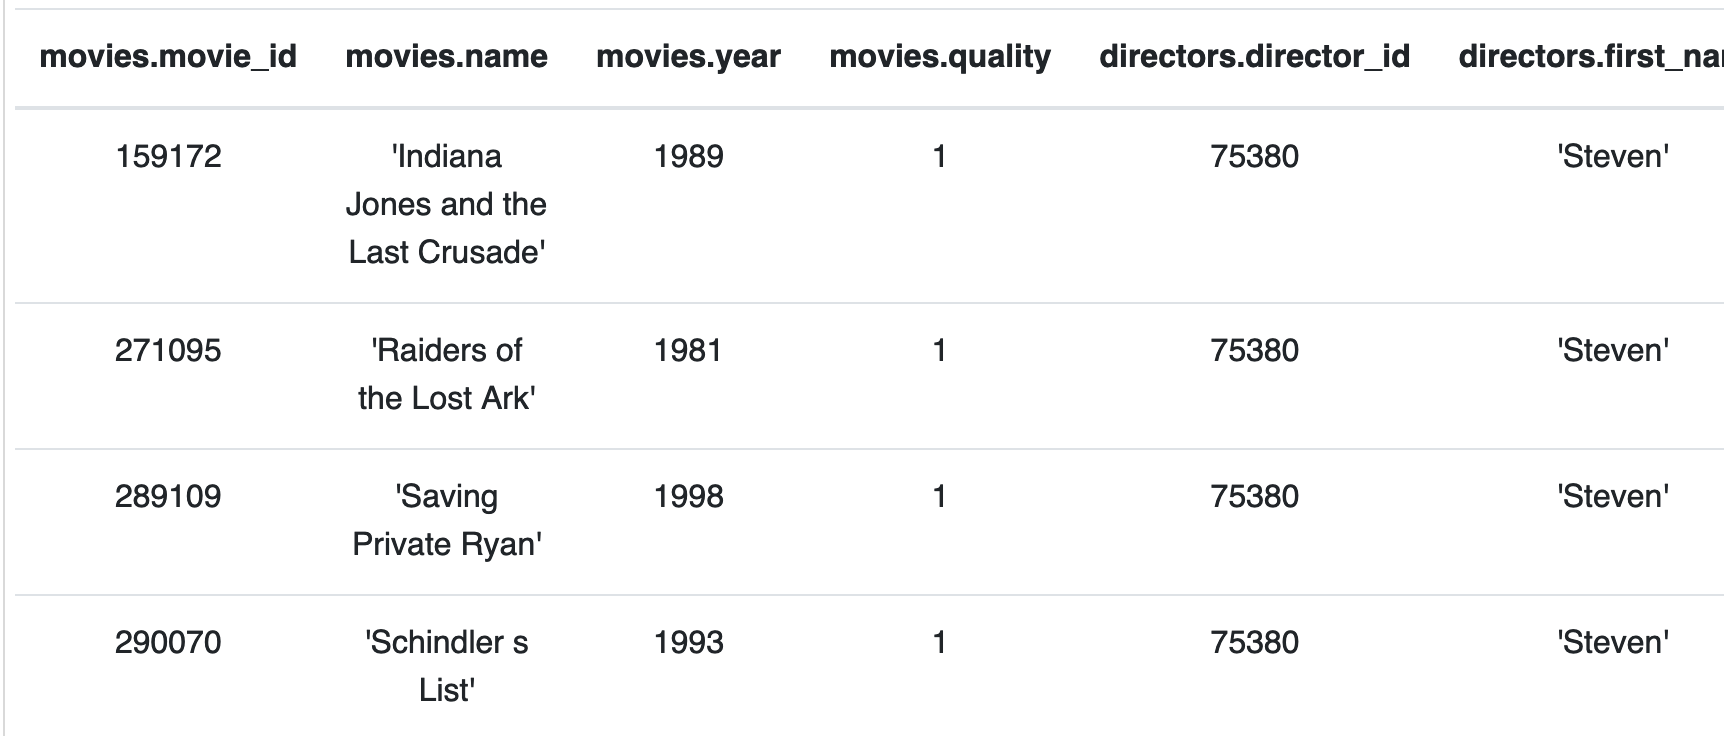
\includegraphics[width=0.7\textwidth]{Parcialito3/result1}
\end{figure}

\begin{minted}[mathescape=true,escapeinside=||,breaklines,frame=single]{text}
life_of_brian = |$\rho$| movie_id |$\leftarrow$| id (|$\sigma$| movies.name = 'Life of Brian' movies)
actores_life_of_brian = |$\pi$| roles.actor_id (roles |$\bowtie$| life_of_brian)
actores_life_of_brian_peliculas = |$\rho$| id |$\leftarrow$| roles.movie_id (|$\pi$| roles.movie_id (actores_life_of_brian |$\bowtie$| roles))

|$\pi$| movies.name (actores_life_of_brian_peliculas |$\bowtie$| movies)
\end{minted}

\begin{figure}[H]
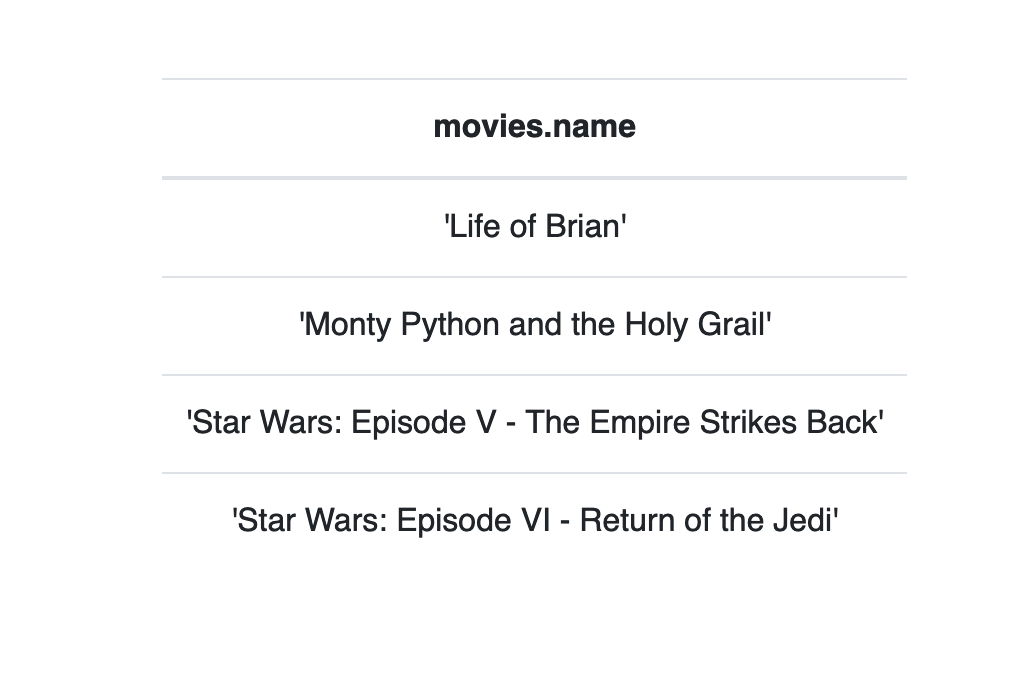
\includegraphics[width=0.7\textwidth]{Parcialito3/result2}
\end{figure}

\begin{minted}[mathescape=true,escapeinside=||,breaklines,frame=single]{text}
id_birgman = |$\rho$| director_id |$\leftarrow$| id (|$\sigma$| directors.first_name = 'Ingmar' |$\land$|  directors.last_name = 'Bergman' directors)
peliculas_bergman = |$\rho$| movie_id |$\leftarrow$| id (|$\pi$| movies.id (movies |$\bowtie$| id_birgman))
actores_bergman = |$\rho$| id |$\leftarrow$| actor_id (|$\pi$| roles.actor_id (roles |$\bowtie$| peliculas_bergman))

actors |$\bowtie$| actores_bergman
\end{minted}

\begin{figure}[H]
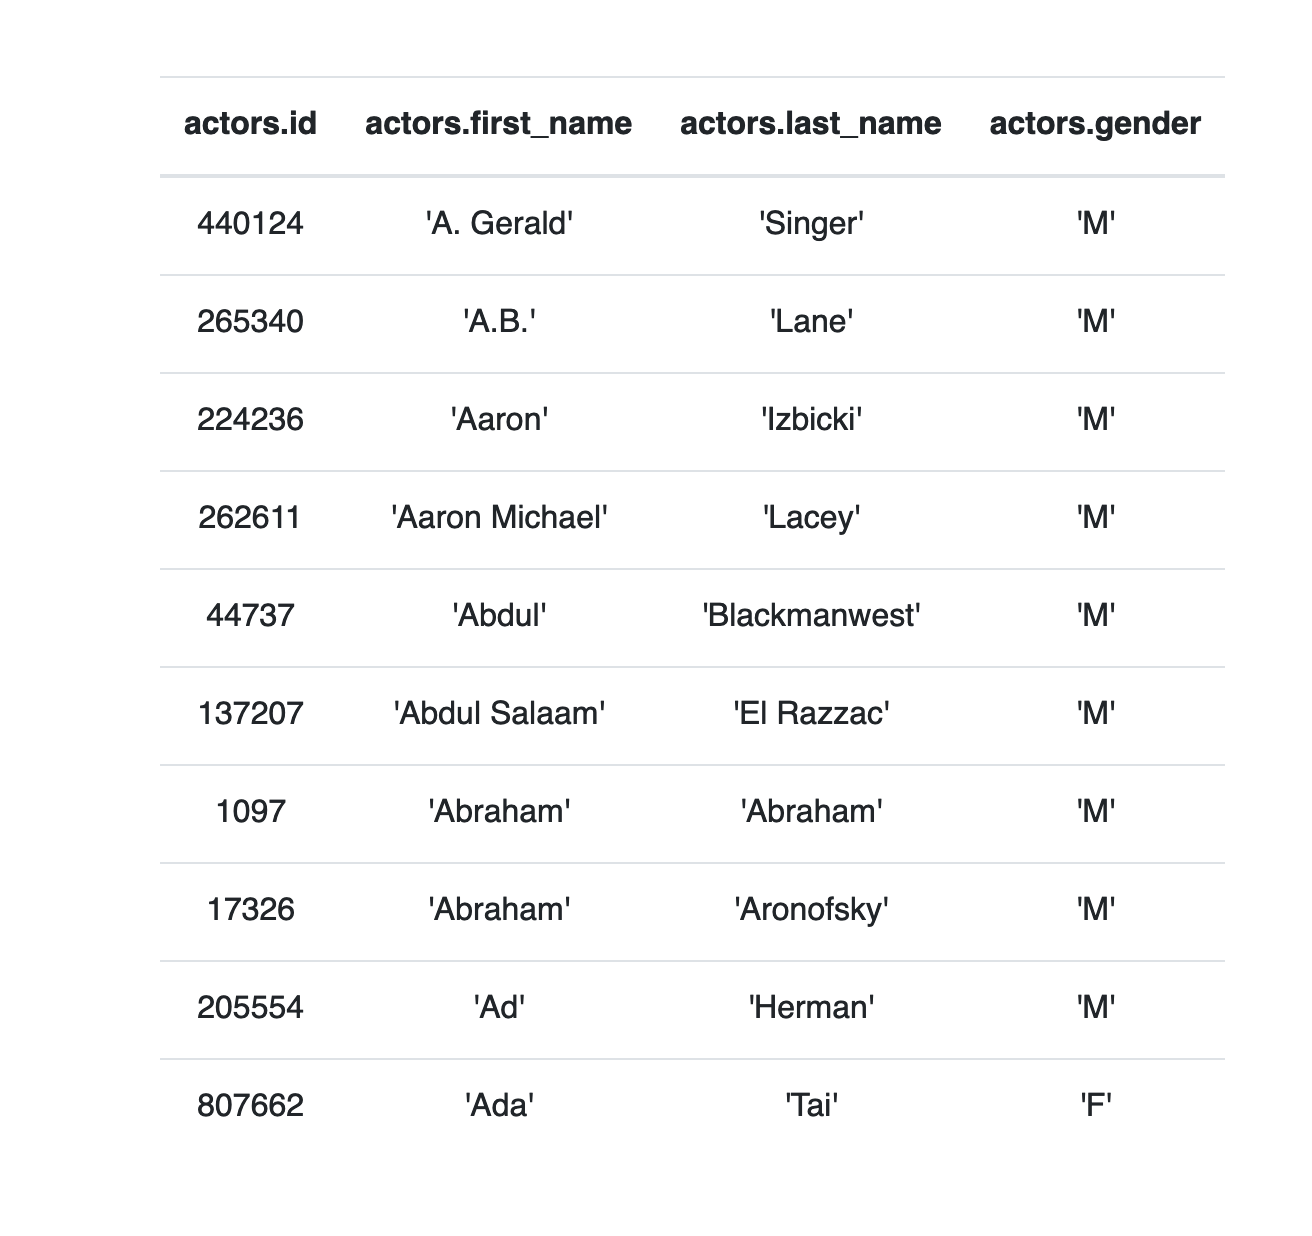
\includegraphics[width=0.7\textwidth]{Parcialito3/result3}
\end{figure}

\begin{minted}[mathescape=true,escapeinside=||,breaklines,frame=single]{text}
war_movies = |$\rho$| id |$\leftarrow$| movies_genres.movie_id (|$\pi$| movies_genres.movie_id (|$\sigma$| movies_genres.genre = 'War' movies_genres)) |$\bowtie$| movies

war_years_1 = |$\pi$| year_1 (|$\rho$| year_1 |$\leftarrow$| movies.year (war_movies))
war_years_2 = |$\pi$| year (war_movies)
war_young_years = |$\pi$| year_1 (|$\sigma$| year_1 > year (war_years_1 ⨯ war_years_2))

war_oldest_year = war_years_2 - war_young_years

war_oldest_movies = |$\rho$| movie_id |$\leftarrow$| id (war_movies |$\bowtie$| war_oldest_year)
war_oldest_movies_actors = actors |$\bowtie$| (|$\rho$| id |$\leftarrow$| roles.actor_id (|$\pi$| roles.actor_id, movies.name (roles |$\bowtie$| war_oldest_movies)))

|$\pi$| actors.first_name, actors.last_name, movies.name (war_oldest_movies_actors)
\end{minted}

\begin{figure}[H]
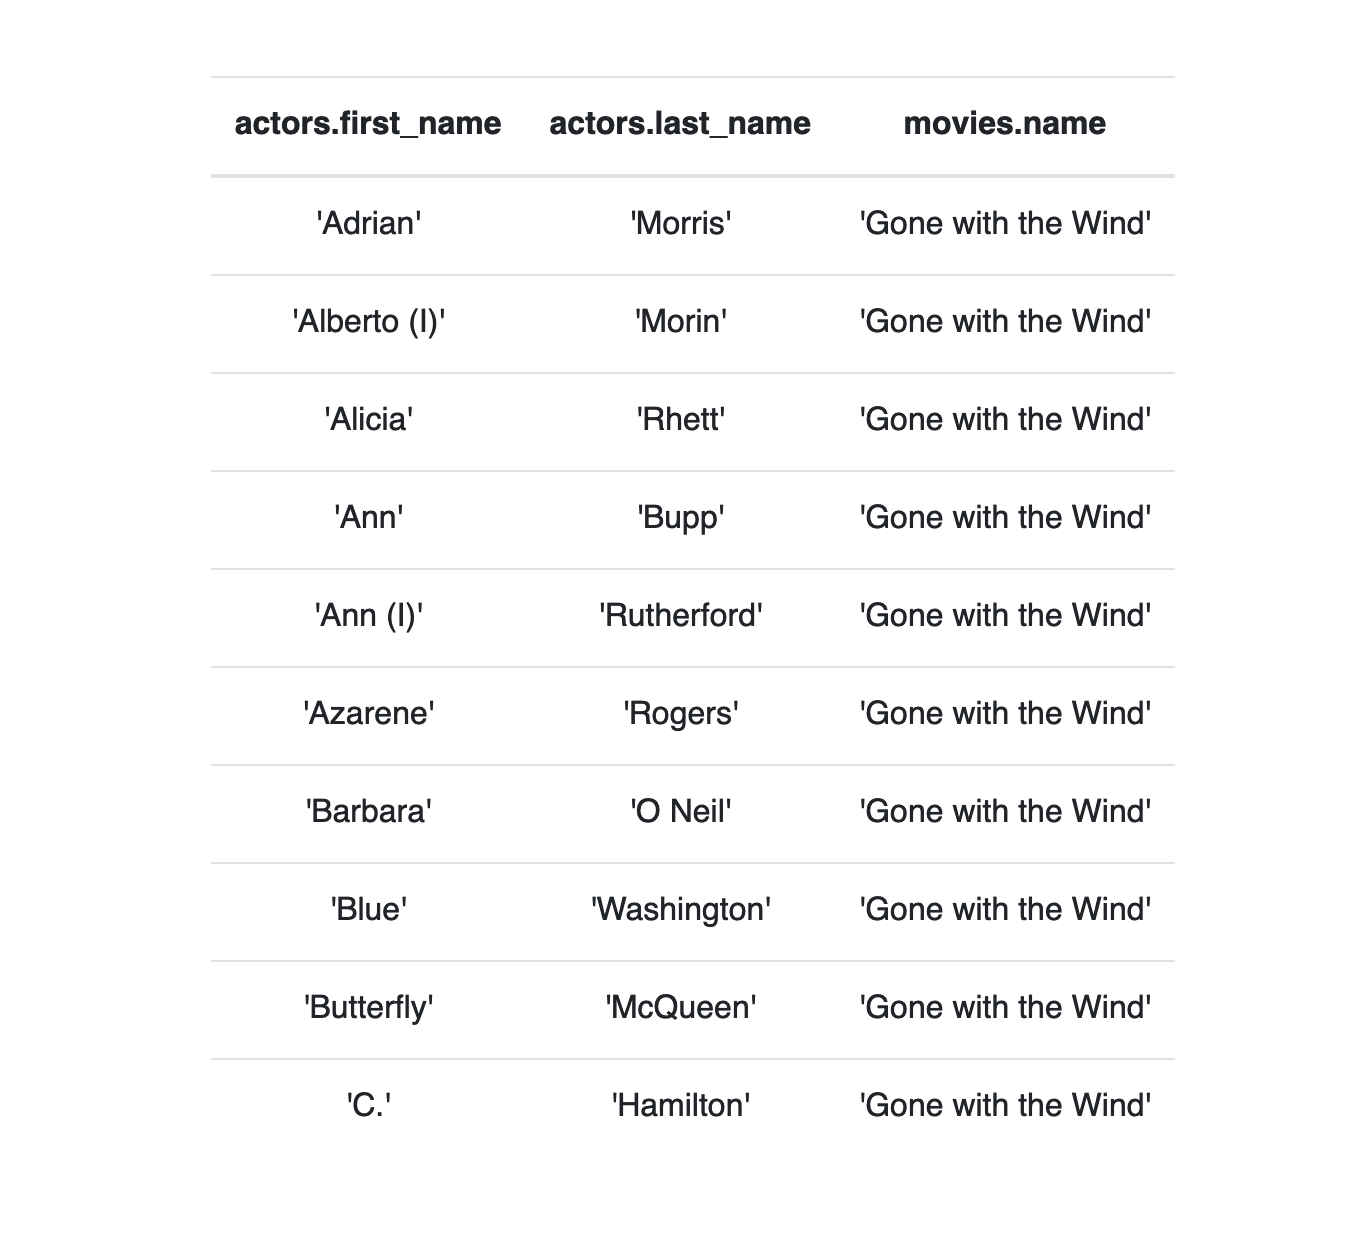
\includegraphics[width=0.7\textwidth]{Parcialito3/result4}
\end{figure}

\begin{minted}[mathescape=true,escapeinside=||,breaklines,frame=single]{text}
genres_0 = |$\pi$| movie_id, genre (movies_genres)
genres_1 = |$\rho$| genre_1|$\leftarrow$|genre ( |$\pi$| movie_id, genre (movies_genres))
genres_2 = |$\rho$| genre_2|$\leftarrow$|genre ( |$\pi$| movie_id, genre (movies_genres))

|$\pi$| movie_id (|$\sigma$| genre != genre_1 |$\land$|  genre != genre_2 |$\land$|  genre_1 != genre_2  (genres_0 |$\bowtie$| genres_1 |$\bowtie$| genres_2))
\end{minted}

\begin{figure}[H]
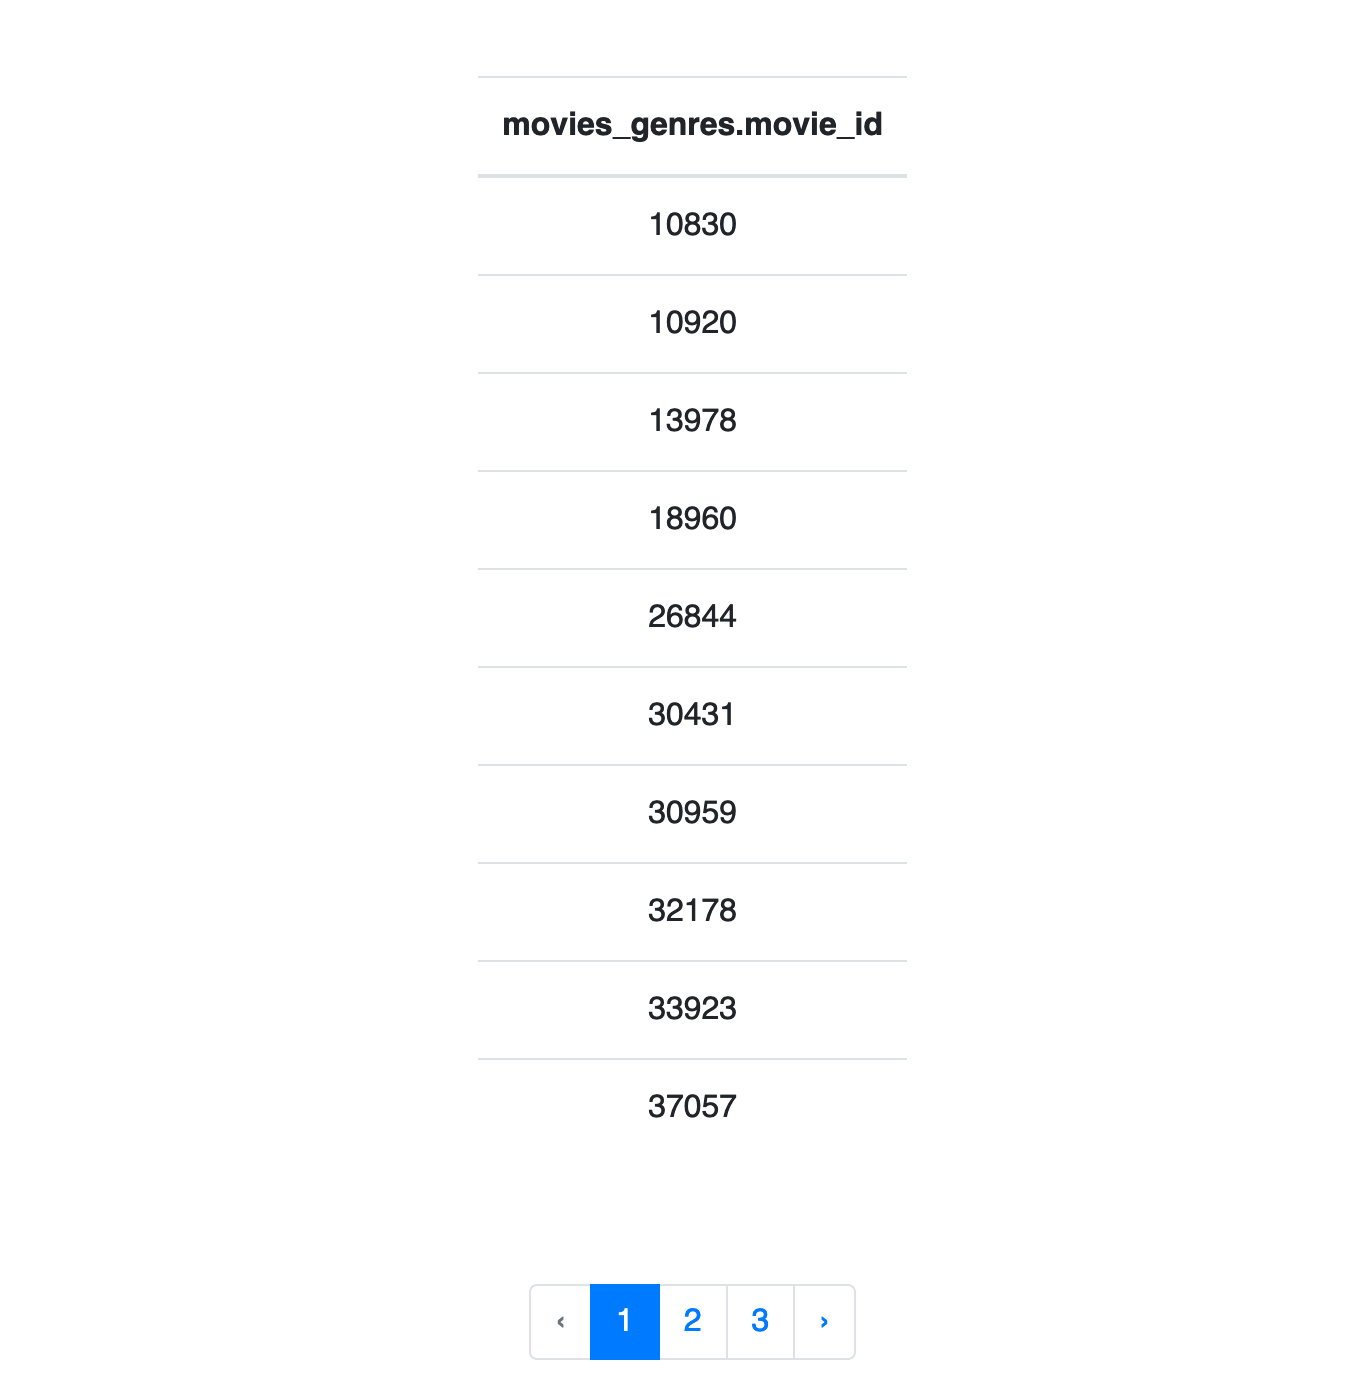
\includegraphics[width=0.7\textwidth]{Parcialito3/result5}
\end{figure}

\end{document}
